\documentclass[14pt]{extbook}
\usepackage{multicol, enumerate, enumitem, hyperref, color, soul, setspace, parskip, fancyhdr} %General Packages
\usepackage{amssymb, amsthm, amsmath, latexsym, units, mathtools} %Math Packages
\everymath{\displaystyle} %All math in Display Style
% Packages with additional options
\usepackage[headsep=0.5cm,headheight=12pt, left=1 in,right= 1 in,top= 1 in,bottom= 1 in]{geometry}
\usepackage[usenames,dvipsnames]{xcolor}
\usepackage{dashrule}  % Package to use the command below to create lines between items
\newcommand{\litem}[1]{\item#1\hspace*{-1cm}\rule{\textwidth}{0.4pt}}
\pagestyle{fancy}
\lhead{Module11L}
\chead{}
\rhead{Version C}
\lfoot{5317-4125}
\cfoot{}
\rfoot{test}
\begin{document}

\begin{enumerate}
\item{
List 10 numbers you should use to estimate the one-sided limit of the function below as $x$ approaches 4 from the right.\[ \frac{\frac{4}{x} - 1}{x - 4} \]} \newpage
\item{
Evaluate the limit below, if possible.\[ \lim_{x \rightarrow 8} \frac{\sqrt{7x - 40} - 4}{3x - 24} \]} \newpage
\item{
Based on the information below, what can be said about (a.) $f(8)$ and (b.) $f(x)$ when $x$ is close to $8$?
\begin{center}
    \textit{ As $x$ approaches $8$, $f(x)$ approaches $13.449$. }
\end{center}
} \newpage
\item{
For the graph below, find the value(s) $a$ that makes the statement true: $ \displaystyle \lim_{x \rightarrow a} f(x) = -\infty$.
\begin{center}
    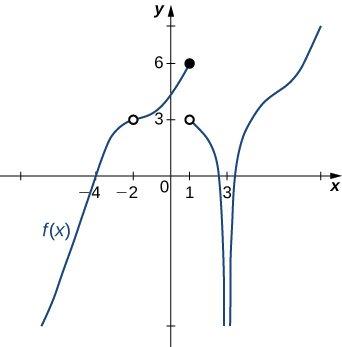
\includegraphics[width=0.5\textwidth]{../Figures/evaluateLimitGraphicallyC.png}
\end{center}
} \newpage
\item{
List 10 numbers you should use to estimate the one-sided limit of the function below as $x$ approaches 10 from the right.\[ \frac{\frac{10}{x} - 1}{x - 10} \]} \newpage
\item{
Based on the information below, what can be said about (a.) $f(3)$ and (b.) $f(x)$ when $x$ is close to $3$?
\begin{center}
    \textit{ $f(x)$ approaches $\infty$ as $x$ approaches $3$. }
\end{center}
} \newpage
\item{
Evaluate the one-sided limit of the function $f(x)$ below, if possible.\[ \lim_{x \rightarrow -4^-} \frac{4}{(x+4)^7}+4 \]} \newpage
\item{
For the graph below, find the value(s) $a$ that makes the statement true: $ \displaystyle \lim_{x \rightarrow a} f(x) = 0$.
\begin{center}
    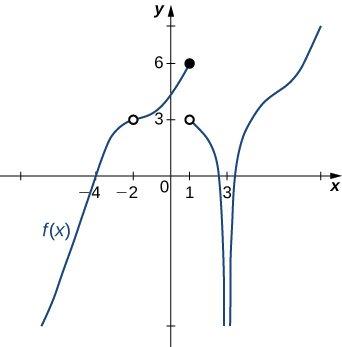
\includegraphics[width=0.5\textwidth]{../Figures/evaluateLimitGraphicallyCopyC.png}
\end{center}
} \newpage
\item{
Evaluate the limit below, if possible.\[ \lim_{x \rightarrow 4} \frac{\sqrt{8x - 16} - 4}{7x - 28} \]} \newpage
\item{
Evaluate the one-sided limit of the function $f(x)$ below, if possible.\[ \lim_{x \rightarrow -4^-} \frac{7}{(x+4)^8}+1 \]} \newpage
\end{enumerate}

\end{document}